%++++++++++++++++++++++++++++++++++++++++
% Don't modify this section unless you know what you're doing!
\documentclass[letterpaper,12pt]{article}

\usepackage{comment}
%\usepackage{hyperref}
\usepackage{parskip}
\usepackage{tabularx} % extra features for tabular environment
\usepackage{amsmath}  % improve math presentation
\usepackage{graphicx} % takes care of graphic including machinery
\usepackage[margin=1in,letterpaper]{geometry} % decreases margins
\usepackage{cite} % takes care of citations
\usepackage[final]{hyperref} % adds hyper links inside the generated pdf file
\hypersetup{
	colorlinks=true,       % false: boxed links; true: colored links
	linkcolor=blue,        % color of internal links
	citecolor=blue,        % color of links to bibliography
	filecolor=magenta,     % color of file links
	urlcolor=blue         
}
%++++++++++++++++++++++++++++++++++++++++


\begin{document}

\title{Handle Multilinguality in Text classification}

\author{Nesma Mahmoud: B8771\\ Mahmoud Shoush: B87770\\ [1cm]{\small Natural language processing (LTAT.01.001) - Spring 2019}}

%\author{Mahmoud Kamel}
%\date{\today}
\date{\vspace{-5ex}}
\maketitle


\vspace{30 mm}
\begin{abstract}
Text classification is a supervised machine learning method used to classify sentences or text documents into one or more defined categories. It’s a widely used natural language processing task playing an important role in Spam filtering, sentiment analysis, categorization of news articles and many other business related issues. Handling multilinguality in text classification is a crucial process, and there is no standard approach to handle it. In this project we propose and compare between Four different methods to tackle the multilinguality in text classification (MLTC): \\

$\bullet$ \textbf{Multiple monolingual classification approach.}

$\bullet$ \textbf{Comparing joint multilingual approach.}

$\bullet$ \textbf{Joint translated monolingual.}

$\bullet$ \textbf{Round trip translation.}\\

We did experiments using different models, and find the round trip translation is the best one to handle MLTC. \textbf{Still need more explanation}.


\end{abstract}

\begin{figure*}
	\centering
	\begin{minipage}[b]{.4\textwidth}
		\centering 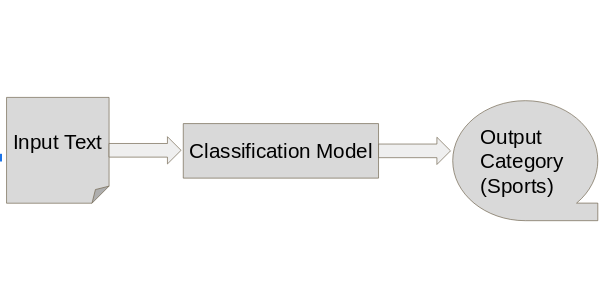
\includegraphics[width=0.8\columnwidth]{sport.png}
		
		\caption{
			\label{fig:1} % spaces are big no-no withing labels
			Text Classification
		}
		
	\end{minipage}\qquad
	\begin{minipage}[b]{.4\textwidth}
		
		\centering 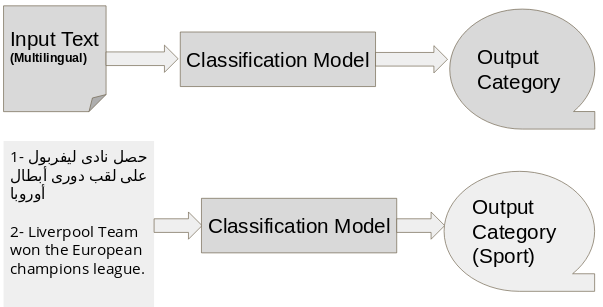
\includegraphics[width=0.8\columnwidth]{2.png}
		
		\caption{
			\label{fig:2} % spaces are big no-no withing labels
			Multilingual Text Classification.
		}
		
	\end{minipage}
\end{figure*}


\section{Introduction}
Natural Language Processing (NLP) is the technology used to teach computers to understand and generate the human’s natural language. NLP is the driving force behind abundance set of applications such as, language translation applications like Watson IBM, Word Processors such as Microsoft Word and Grammarly that employ NLP to check grammatical accuracy of texts, and 
Personal assistant applications such as OK Google, Siri, Cortana, and Alexa etc. There are many approaches to automatic text classification, which can be grouped into three different types of systems, Rule-based systems, Machine Learning based systems, and Hybrid systems. 


Text classification is one of the major tasks in NLP (a.k.a. text categorization or text tagging) is the task of assigning a set of predefined categories to free-text. Text classification can be used to organize, structure, and categorize pretty much anything. For example, new articles can be organized by topics, support tickets can be organized by urgency, chat conversations can be organized by language, brand mentions can be organized by sentiment, and so on. For example (see figure~\ref{fig:3}), imagine you have a text with different categories “European Champions league is a quite hard and tough for many teams.” A classifier can take this text as an input, analyze its content, and then automatically assign relevant category, such as Sport and tag as difficult. 

Multilingual text classification (MLTC) (see figure~\ref{fig:4}) means collections of documents written in several languages with different set of labels that we need to classify and predict \cite{Teresa_Gonalves}. 


\section{Related Work}
There has been research on MLTC in the case of enough training documents being available for every language. In \cite{Teresa_Gonalves} they proposed a method that combines different monolingual classifiers in order to get a new classifier as good as the best monolingual one which has the ability to deliver all the best performance measures (precision, recall and F1) possible. In \cite{delmo} they provide linguistic arguments against existing approaches and devise a novel solution that exploits background knowledge from ontologies and lexical resources. In \cite{Makoto} They proposed a method which is language-independent because it does not depend on the low of grammar by using Character N-gram. Therefore, they can classify multi-language into some categories using only one program. In \cite{Ruochen} This paper presents a novel approach to Cross-lingual Distillation for Text Classification that builds on model distillation, which adapts and extends a framework originally proposed for model compression. Using soft probabilistic predictions for the documents in a label-rich language as the (induced) supervisory labels in a parallel corpus of documents, we train classifiers successfully for new languages in which labeled training data are not available.




\section{Proposed Approach}
In this section, we will explain in details our proposed approach through the whole four main stages that we mentioned before. The proposed methods have been implemented based on the STOA NLP frameworks such as Bert \cite{bert}, Elmo \cite{elmo}, and Alennlp \cite{allen}. The code and detailed implementation can be found in \href{https://github.com/nesmaAlmoazamy/Handling_Multilinguality }{Handling\_Multilinguality repo}. For this project we find a  
 \href{https://github.com/valeriano-manassero/multilingual-text-categorization-dataset}{multilingual-text-categorization-dataset} that contains 33 languages and 45 categories. After exploring the dataset we discovered that it's not balanced (some of the languages are more bigger than the others), and for this project we used only five languages (English, Arabic, French, Spanish, and Estonian).




\begin{figure*}
	\centering
	\begin{minipage}[b]{.4\textwidth}
		\centering 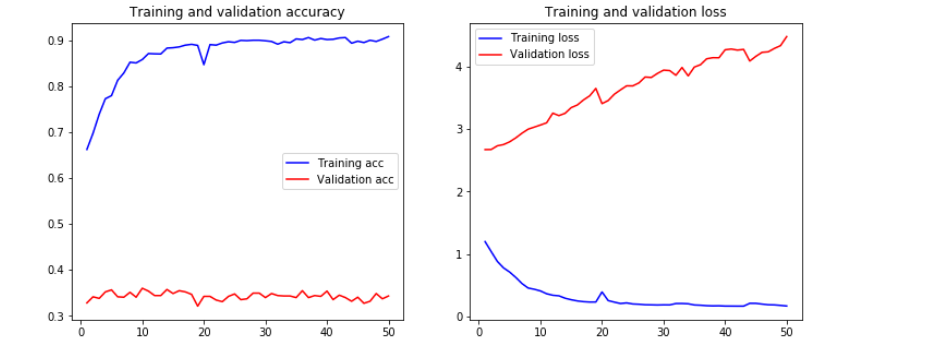
\includegraphics[width=0.8\columnwidth]{w.png}
		
		\caption{
			\label{fig:3} % spaces are big no-no withing labels
			Text classification with preprocessing
		}
		
	\end{minipage}\qquad
	\begin{minipage}[b]{.4\textwidth}
		
		\centering 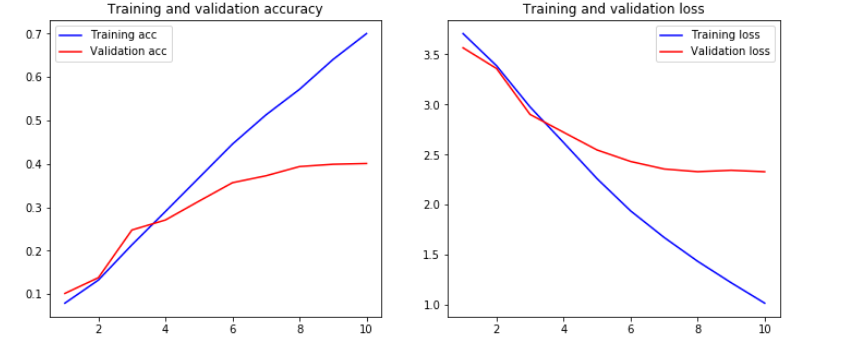
\includegraphics[width=0.8\columnwidth]{without.png}
		
		\caption{
			\label{fig:4} % spaces are big no-no withing labels
			Text Classification without preprocessing.
		}
		
	\end{minipage}
\end{figure*}



\subsection{Text Preprocessing}
In this section, we will talk about the basic steps of \href{https://github.com/nesmaAlmoazamy/Handling_Multilinguality/blob/master/EnglishData_classification_with_preprocessing.ipynb}{text preprocessing}. These steps are needed for transferring text from human language to machine-readable format for further processing. After a text is obtained, we start with text normalization. Text normalization includes converting all letters to lower case, remove stop words, numbers, punctuation, blank space, and URL, stemming, and lemmatization. This dataset contains blog posts labeled by language and by category.

In this step we used a Keras framework to build our classifier and apply it on EnglishData only with/without preprocessing, (see figure~\ref{fig:3}) and (\ref{fig:4}) respectively. We can see obviously that heavy preprocessing gives negative impact on the classification process. Here can check the implementation of 
\href{https://github.com/nesmaAlmoazamy/Handling_Multilinguality/blob/master/EnglishData_classification_with_preprocessing.ipynb}{with preprocessing}, and \href{https://github.com/nesmaAlmoazamy/Handling_Multilinguality/blob/master/EnglishData_Classification_without_preprocessing.ipynb}{without pre-processing}.



\subsection{Multiple Monolingual Classification}
This is the first method to tackle the the MLTC problem. In this approach we classify all of the languages (English, Arabic, French, Spanish, and Estonian) by a separate classification model (see figure~\ref{fig:5}) using different models such as Flair, and Allennlp. 
\href{https://github.com/nesmaAlmoazamy/Handling_Multilinguality/blob/master/AllenNlp_SingleClassifier_All_RoundTrip.ipynb}{Here} you can see check the Allennlp implementation for each language separately. Also we used Flair Embedding and Glove over English dataset with 2 categories as a POC due to resources shortage \href{https://github.com/nesmaAlmoazamy/Handling_Multilinguality/blob/master/FlairEnglishClassificationPOC.ipynb}{here} and when it compares to Allennlp implementation we got accuracy around 65 \% which is an improvement over Allennlp. From this step we find that using Flair has an advantage over Allennlp implementation.




\begin{figure*}
	\centering
	\begin{minipage}[b]{.4\textwidth}
		\centering 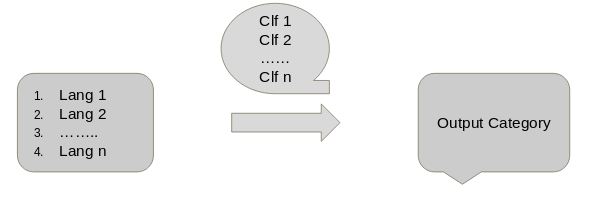
\includegraphics[width=0.8\columnwidth]{4.png}
		
		\caption{
			\label{fig:5} % spaces are big no-no withing labels
			Multiple Monolingual Classification
		}
		
	\end{minipage}\qquad
	\begin{minipage}[b]{.4\textwidth}
		
		\centering 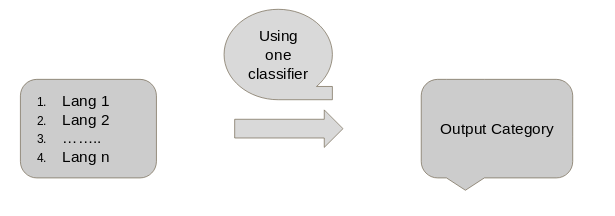
\includegraphics[width=0.8\columnwidth]{3.png}
		
		\caption{
			\label{fig:6} % spaces are big no-no withing labels
			Joint multilingual approach.
		}
		
	\end{minipage}
\end{figure*}

\subsection{Joint multilingual approach}
In the second method that we propose to handle MLTC, we classify all of the languages together with single classification system (see figure~\ref{fig:6}) using different models as the previous step. \href{https://github.com/nesmaAlmoazamy/Handling_Multilinguality/blob/master/AllenNlp_SingleClassifier_All_RoundTrip.ipynb}{here} you cand find the Allennlp implementation for this approach, however in this step all languages are concatenated and the dataset splited into 80\%, 20\% for training step and 20\% from all languages was selected as validation. Also, we did validation using a subset from the English dataset, which was excluded before spliting the whole data frame into train and dev and got accuracy around 75\%. 



\subsection{Joint translated monolingual}
This is the third method that we propose to handle the MLTC problem. In this method all languages are translated into one super-language - English - and then classified all together (see figure~\ref{fig:7}). For this approach we tried to use different public translation service such as \href{https://py-googletrans.readthedocs.io/en/latest/}{googletrans}, and \href{https://www.ibm.com/watson/services/language-translator/}{Watson IBM languge translator}, but in this public services the free usage is so limited per character and per account credentials then accordingly we didn't able to apply this step for the whole dataset however we minimize the number of words per row to fifty words. You can find detailed implementation  \href{https://github.com/nesmaAlmoazamy/Handling_Multilinguality/blob/master/IBMTranslationPOC.ipynb}{here}. \textbf{Add results about accuracy??????}


\begin{figure*}
	\centering
	\begin{minipage}[b]{.4\textwidth}
		\centering 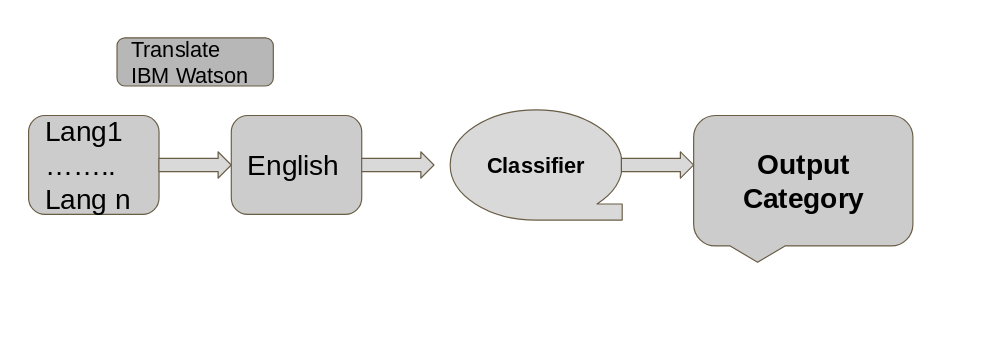
\includegraphics[width=0.8\columnwidth]{trans.png}
		
		\caption{
			\label{fig:7} % spaces are big no-no withing labels
			Joint translated monolingual
		}
		
	\end{minipage}\qquad
	\begin{minipage}[b]{.4\textwidth}
		
		\centering 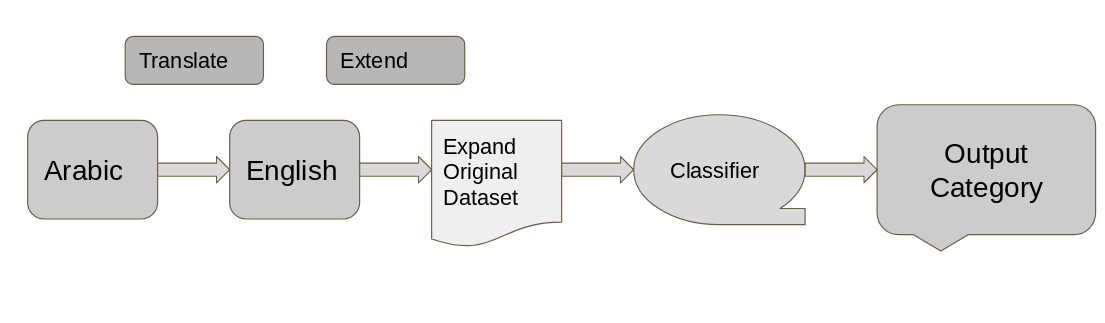
\includegraphics[width=0.8\columnwidth]{5.png}
		
		\caption{
			\label{fig:8} % spaces are big no-no withing labels
			Round Trip Translation.
		}
		
	\end{minipage}
\end{figure*}

\subsection{Round Trip Translation.}
In this last approach we used round trip translation to expand the available data. In this method we translated all languages to English, then add the translated part to the original dataset to expand it, after that apply our classifier to the expanded dataset(see figure~\ref{fig:9}). \href{https://github.com/nesmaAlmoazamy/Handling_Multilinguality/blob/master/AllenNlp_SingleClassifier_All_RoundTrip.ipynb}{Here} you can find the implementation of the RT applied Arabic \textbf{Add other languages} and we got accuracy around 24\%.




\begin{figure*}
	\centering
	\begin{minipage}[b]{.4\textwidth}
		\centering 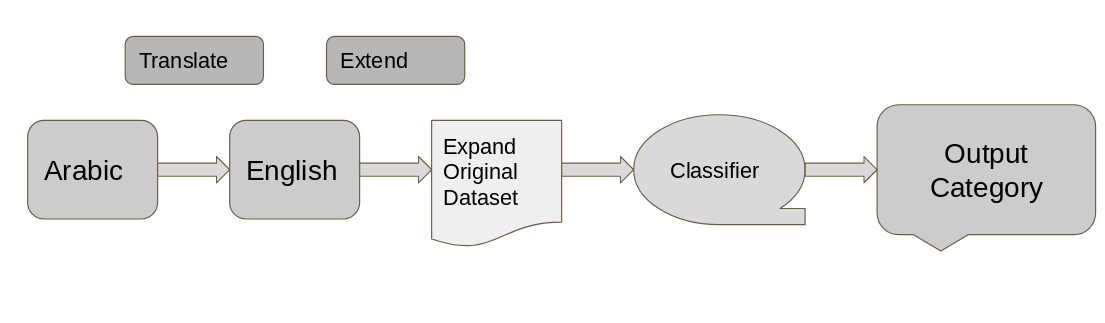
\includegraphics[width=0.8\columnwidth]{5.png}
		
		\caption{
			\label{fig:9} % spaces are big no-no withing labels
			Round Trip Approach
		}
		
	\end{minipage}\qquad
	\begin{minipage}[b]{.4\textwidth}
		
		\centering 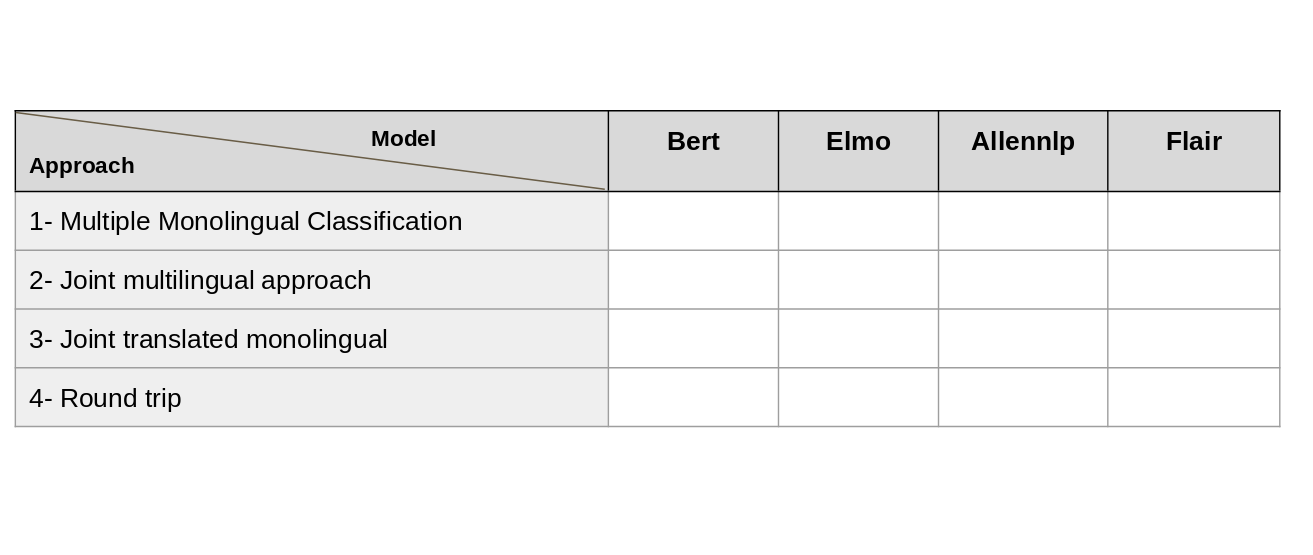
\includegraphics[width=0.8\columnwidth]{6.png}
		
		\caption{
			\label{fig:10} % spaces are big no-no withing labels
			Results conclusion.
		}
		
	\end{minipage}
\end{figure*}


\section{Conclusion and discussion}
In this section we will conclude our experiments and results. We proposed four approaches to tackle the multilinguality in text classification for each approach we used different models frameworks. \textbf{Add explanation after fulfilling the missing results}



\section{Future Work}
This project just a start in MLTC using different models, and there is alot to do to enhance the process of text classification with multilingual languages. In this section I will try to include some ideas to enhance this project. First we need to build a complete dataset for the purpose of MLTC since the available datasets are not balanced and limited to specifics topics and objectives. Also we need to use fee-based service for translation between different languages at the same time to solve the problem of accounts usage. 





\begin{thebibliography}{}
	
\bibitem{Teresa_Gonalves}
Gonalves, T.,\& Quaresma, P. (2010). Multilingual text classification through combination of monolingual classifiers. In Proceedings of the 4th Workshop on Legal Ontologies and Artificial Intelligence Techniques (pp. 29-38).

\bibitem{delmo}
De Melo, G. and Siersdorfer, S., 2007, April. Multilingual text classification using ontologies. In European Conference on Information Retrieval (pp. 541-548). Springer, Berlin, Heidelberg.

\bibitem{Makoto}
Suzuki, Makoto, Naohide Yamagishi, Yi-Ching Tsai, and Shigeichi Hirasawa. "Multilingual text categorization using Character N-gram." In 2008 IEEE Conference on Soft Computing in Industrial Applications, pp. 49-54. IEEE, 2008.

\bibitem{Ruochen}
Xu, Ruochen, and Yiming Yang. "Cross-lingual distillation for text classification." arXiv preprint arXiv:1705.02073 (2017).


\bibitem{bert}
Devlin, Jacob, Ming-Wei Chang, Kenton Lee, and Kristina Toutanova. "Bert: Pre-training of deep bidirectional transformers for language understanding." arXiv preprint arXiv:1810.04805 (2018).

\bibitem{elmo}
Peters, Matthew E., Mark Neumann, Mohit Iyyer, Matt Gardner, Christopher Clark, Kenton Lee, and Luke Zettlemoyer. "Deep contextualized word representations." arXiv preprint arXiv:1802.05365 (2018).

\bibitem{allen}
Gardner, Matt, Joel Grus, Mark Neumann, Oyvind Tafjord, Pradeep Dasigi, Nelson Liu, Matthew Peters, Michael Schmitz, and Luke Zettlemoyer. "AllenNLP: A deep semantic natural language processing platform." arXiv preprint arXiv:1803.07640 (2018).



\end{thebibliography}


\end{document}
